%!TEX program = xelatex
\documentclass[cn,sakura,14pt,screen,bibstyle=gb7714-2015,math=mtpro2]{elegantnote}
\title{双重差分设计}
\date{\today}

\usepackage{array}
\usepackage{geometry}
\usepackage{amsmath, amsthm, amssymb}
\usepackage{cprotect}
\usepackage{array}
\usepackage{bbm}
\usepackage{hyperref}

\newcommand{\E}{\mathbb{E}}
\newcommand{\X}{X}
\newcommand{\overbar}[1]{\mkern 1.5mu\overline{\mkern-1.5mu#1\mkern-1.5mu}\mkern 1.5mu}
\geometry{left=3.17cm,right=3.17cm,top=2.54cm,bottom=2.54cm}
\addbibresource[location=local]{reference.bib}
\begin{document}

\maketitle

\centerline{
  
\includegraphics[width=0.3\textwidth]{Logo.png}
}



\section{经典双重差分}

假设$D_i\in \{0,1\}$表示处置(treatment), 表示个体$i$是否接受处置(参加培训), 其中1代表接受处置(个体$i$位于处置组), 0代表没有接受处置(个体$i$位于控制组).


假设$Y_i$代表结果变量(outcome), $Y_{i,t}(0,0)$表示个体$i$在$t$时刻的\textbf{潜在结果} (potential outcome), 如果$i$在两个时期都保持未处置. 类似地, $Y_{i,t}(0,1)$表示个体$i$在$t$时刻的潜在结果, 如果$i$在第一期未处置而在第二期接受处置.

为了简化符号, 记$Y_{i,t}(0)=Y_{i,t}(0,0)$以及$Y_{i,t}(1)=Y_{i,t}(0,1)$. 由于因果推断的根本问题, 我们实际上只能观测到
$$Y_{i,t}=D_iY_{i,t}(1)+(1-D_i)Y_{i,t}(0)$$
换言之, 一旦个体$i$接受处置, 那就无法观测到它未接受处置的\textbf{反事实结果} (counterfactual outcome), 反之亦然.

在本文剩余部分, 我们均给定\textbf{个体稳定处置效应假设} (Stable Unit Treatment Value Assumption, SUTVA)成立, 也即任何个体的潜在结果不随其它个体是否接受处置而变化, 并且每一个体所接受的处置水 平是唯一的, 因此处置所导致的潜在结果也是唯一的.

在政策评估领域, 研究者感兴趣的因果效应为
$$\tau_2=\E[Y_{i,2}(1)-Y_{i,1}(0)|D_i=1]$$
它衡量了接受处置的个体在接受处置时 ($t=2$)的平均因果效应, 称之为\textbf{处置组平均处置效应} (Average Treatment Effect on the Treated, ATT). 为了正确识别和估计$\tau_2$, 可以使用\textbf{双重差分法} (Difference-in-Differences, DiD).

在SUTVA成立的情况下, ATT是良好定义的, 但由于反事实结果的存在, 我们仍然无法识别出它. 换言之, 为了正确识别ATT, 还需要准备其它假设条件.

\begin{definition}[平行趋势]
  $\E[Y_{i,2}(0)-Y_{i,1}(0)|D_i=1]=\E[Y_{i,2}(0)-Y_{i,1}(0)|D_i=0]$.
\end{definition}
平行趋势假设意味着, 如果没有政策冲击, 那么处置组和控制组中的平均结果变量随时间变化的趋势是平行的. 换言之, 其他因素造成的影响处置的\textbf{选择偏差} (selection bias)在$t=1$和$t=2$是相同的.

\begin{definition}[无预期效应]
对于所有$D_i=1$的个体$i$都有$Y_{i,1}(0)=Y_{i,1}(1)$.
\end{definition}
无预期效应意味着, 在政策冲击到来之前, 没有任何处置组中的个体会预期到它的到来而作出反应. 换言之, 政策冲击在实施前对结果变量没有任何因果效应.

如果平行趋势和无预期效应成立, 那么在$t=2$时刻的处置组平均处置效应$\tau_2$可以被成功识别, 经过简单的数学运算可得
$$\tau_2=\E[Y_{i,2}(1)-Y_{i,1}(1)|D_i=1]-\E[Y_{i,2}(0)-Y_{i,1}(0)|D_i=0]$$
上式第1项表示由于政策冲击和其他因素造成的处置组结果变量的平均差异, 第2项为其他因素造成的控制组结果变量的平均差异, 因此该方法称为双重差分.

现在已经正确识别出了$\tau_2$, 一个估计它的自然想法是用样本均值替代期望, 得到
$$\hat{\tau}_2=(\overbar{Y}_{t=2,d=1}-\overbar{Y}_{t=1,d=1})-(\overbar{Y}_{t=2,d=0}-\overbar{Y}_{t=1,d=0})$$
其中$\overbar{Y}_{t=t',D=d}$是组别$d$中的$Y$在$t'$时刻的样本均值. 另一方面, 还可以使用双向固定效应 (Two-Way Fixed Effects, TWFE)回归
$$Y_{i,t}=\alpha_i+\phi_t+(1[t=2]\cdot D_i)\beta+\epsilon_{i,t}$$
可以证明$\beta$的OLS估计量$\hat{\beta}$等于$\hat{\tau}_2$. 最后, 我们可以在TWFE中加入不受处置影响的协变量$X$得到
$$Y_{i,t}=\alpha_i+\phi_t+(1[t=2]\cdot D_i)\beta+{X}_{i,t}'\gamma+\epsilon_{i,t}$$
这样可以控制处置组与控制组中随时间变化的可观测特征差异可能导致的估计误差.

\begin{figure}
  \centering
  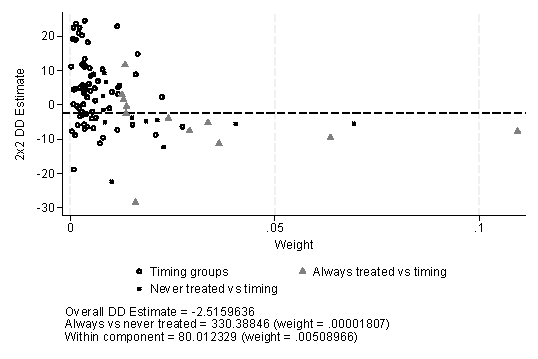
\includegraphics[width=15cm]{Figure3.pdf}
  \caption{双重差分示意图}
\end{figure}
\newpage
\section{交错时间处置}
\subsection{TWFE-DiD估计量的缺陷}
在经典DiD的框架下, 政策在同一时刻发生, 且只包含了处置组和控制组, 然而政策可能具有滞后性, 因此经典DiD不再适用. 有鉴于此, 我们可以将$2\times2$的经典DiD推广至多维, 也即存在多个组群在不同时点受到政策冲击.

假设时间跨度为$T+1$, 每个时点由$t=0,\cdots,T$标记, 个体$i$可以在任意$t\ge0$的时点受到二元处置, 并且处置是\textbf{吸收态} (absorbing state), 也即一旦个体接受处置, 那么它在剩余的时间上保持被处置的状态. 我们使用$D_{i,t}$作为个体$i$在时点$t$是否接受处置的二元指示符, $G_i=\min\{t:D_{i,t}=1\}$为个体$i$首次接受处置的时点, $G_i=\infty$表示个体$i$从未接受处置. 由于处置是吸收的, 因此对于一切$t\ge G_i$都有$D_{i,t}=1$.

我们需要推广潜在结果的表示方法. 设$\mathbf{0}_s$和$\mathbf{1}_s$分别为$s$维的0向量和1向量, 如果个体$i$在时点$g$首次接受处置, 那么它在$t$时刻的潜在结果为$Y_{i,t}(\mathbf{0}_{g-1},\mathbf{1}_{T-g+1})$, 而用$Y_{i,t}(\mathbf{0}_T)$表示从未接受处置的潜在结果, 分别简写为$Y_{i,t}(g)$以及$Y_{i,t}(\infty)$, 并且
$$Y_{i,t}(g)=Y_{i,t}(\infty)+\sum_{0\leq g\leq T}\,[Y_{i,t}(g)-Y_{i,t}(\infty)]\cdot 1[G_i=g]$$

同样地, 为了使用DiD, 我们需要新的平行趋势和无参与效应的假设, 它们是前文所述假设的推广.
\begin{definition}[平行趋势]
对于一切$t\neq t'$, $g\neq g'$都有
$$\E[Y_{i,t}(\infty)-Y_{i,t'}(\infty)|G_i=g]=\E[Y_{i,t}(\infty)-Y_{i,t'}(\infty)|G_i=g']$$
\end{definition}
上式表示, 不管个体$i$在何时接受处置, 如果它们从未接受处置, 那么它在任意时点上的潜在结果将具有平行趋势.

\begin{definition}[无参与效应]
对于一切$i$和$t<g$都有$Y_{i,t}(g)=Y_{i,t}(\infty)$.
\end{definition}

在以上假设成立的情况下, 仍然考虑使用TWFE模型
$$Y_{i,t}=\alpha_i+\phi_t+D_{i,t}\beta_\text{post}+\epsilon_{i,t}$$
如果处置效应跨个体和时间维度没有异质性, 那么使用$\beta$来识别因果是合理的. 正式地说, 定义$\tau_{i,t}(g)=Y_{i,t}(g)-Y_{i,t}(\infty)$, 假设对于一切$i$, 如果当$t\ge g$时有$\tau_{i,t}(g)=\tau$, 那么回归系数$\beta_{\text{post}}$等于$\tau$. 上述同质性处置效应假设表明: (a) 所有的个体受到了相同的处置效应, (b)无论处置开始于何时, 处置具有相同的效应.

值得注意的是, 如果在不同时点受到的处置效应存在异质性, 那么TWFE估计是有偏的 (Goodman-Bacon, 2021), 甚至会出现完全相反的因果效应.

为了看到这一点, 假设$\tau_{i,t}(g)=\sum_{s\ge0}\tau_s1[t-g=s]$, 于是当所有个体接受处置后, 在时点$s$处具有处置效应$\tau_s$, 此时$\beta_\text{post}=\sum_s\omega_s\tau_s$, 权重$\omega_s$之和为1但有可能为负. 此时问题将会出现, 例如所有的$\tau_s$均为正值, 但$\beta_\text{post}$却为负.

事实上, 根据FWL定理可知$\hat{\beta}_{\text{post}}$的OLS估计量为
$$\hat{\beta}_\text{post}=\frac{\sum_{i,t}(D_{i,t}-\hat{D}_{i,t})Y_{i,t}}{\sum_{i,t}(D_{i,t}-\hat{D}_{i,t})^2}$$
其中$\hat{D}_{i,t}$是出自回归$D_{i,t}=\tilde{\alpha}_i+\tilde{\phi}_t+u_{i,t}$的$D_{i,t}$的拟合值. 由于上式分母始终为正, 以及$Y_{i,t}=Y_{i,t}(\infty)+\tau_{i,t}(g)$, 因此如果$D_{i,t}=1$且$D_{i,t}-\hat{D}_{i,t}<0$, 那么$\tau_{i,t}(g)$在$\hat{\beta}_\text{post}$中取得负权重, 即使个体$i$在$t$时刻接受处置.

进一步, 经过某些代数运算可得
$$\hat{D}_{i,t}=\overbar{D}_i+\overbar{D}_t-\overbar{D}$$
其中$\overbar{D}_i=T^{-1}\sum_t D_{i,t}$表示个体$i$的处置$D$在时间上的平均, $\overbar{D}_t=N^{-1}\sum_i D_{i,t}$表示时点$t$的处置$D$在截面上的平均, $\overbar{D}=(NT)^{-1}\sum_{i,t}D_{i,t}$表示处置$D$在整个截面和时间上的平均.

如果个体在几乎所有时点都是处置状态, 那么$\overbar{D}_i\approx 1$, 如果某时点几乎所有个体都被处置, 那么$\overbar{D}_t\approx 1$, 在二者同时成立的情况下有$\hat{D}_{i,t}\approx 2-\overbar{D}$, 如果在某段时间内有部分未接受处置的个体存在, 那么$\hat{D}_{i,t}>1$. 由此可见, 早期接受处置的个体在后期更容易产生负权重.

另一方面, Goodman-Bacon (2021)指出, TWFE-DiD估计量是所有可能的$2\times 2\,$DiD估计量的加权平均, 各个小的DiD估计量的处置组和控制组是混乱的, 有的将从未接受处置的组群作为控制组, 有的将尚未处置 (not-yet-treated)的组群作为控制组, 还有的将先接受处置的组群作为控制组而将后接受处置的组作为处置组. 当存在随时间变化的处置效应异质性时, 某些小的DiD估计量就会产生负权重. 特别地, 使用较早接受处置的组作为控制组被称为禁止比较 (forbidden comparison).

为了解决异质性处置效应下的TWFE-DiD估计偏误, 一方面可以在无异质性处理路径的情况下使用\textbf{事件研究法} (event study method), 另一方面则是使用更具有普适性的稳健的DiD估计量, 下面将分别介绍.
\subsection{事件研究法}
既然情况已经由$2\times 2\,$DiD扩展到了更一般的多个处置时点, 为了利用更多信息, 一个自然考虑是使用动态模型.

假设数据结构为平衡面板数据, 包含个体$i\in\{1,\cdots,N\}$, 每个个体可观测时期为$t\in\{0,\cdots,T\}$, 个体$i$接受处置的时期为$G_i$, 如果从未接受处置则$G_i=\infty$, 个体$i$关于$G_i$的相对处置时间变量为$D_{i,t}=1[t-G_i=l]$, 其中$l$表示相对处置时点, 此外还定义集合$e$, 使得
$$1[t-G_i\in e]=\sum_{l\in e}1[t-G_i=l]=\sum_{l\in e}D_{i,t}^l$$
以及关于相对处置时点$l\in [-T,T]$的互不相交的$e$构成的集族$\mathcal{E}$.

实践中通常考虑如下动态TWFE模型
$$Y_{i,t}=\alpha_i+\phi_t+\sum_{l=-K}^{-2}\mu_lD_{i,t}^l+\sum_{l=0}^{L}\mu_lD_{i,t}^l+\epsilon_{i,t}$$
其中相对时间变量$D_{i,t}$被分为了两组, 一组代表处置前 ($l\leq-2$), 一组代表处置后 ($l\ge0$), 各个$\mu_g$体现了动态效应 (dynamic effects). 此外, 为了避免完全多重共线性, 选取$l=-1$作为基期. 这里的$K=G^{\max}-1$, $L=T-G^{\min}$, 并且$G^{\max}$和$G^{\min}$分别表示最晚和最早接受处置的时间.

Sun and Abraham (2021)证明了, 再无需任何假设的情况下, $\mu_g$可以被分解为
\begin{align*}
\mu_g&=\sum_{l\in e}\sum_{g\neq\infty}w_{g,l}^e(\E[Y_{i,g+l}-Y_{i,0}(\infty)|G_i=g]-\E[Y_{i,g+l}-Y_{i,0}(\infty)]) \\
&\quad+\sum_{e'\neq e,e'\in\mathcal{E}}\sum_{l\in e'}\sum_{g\ne\infty}w_{g,l}^e(\E[Y_{i,g+l}-Y_{i,0}(\infty)|G_i=g]-\E[Y_{i,g+l}-Y_{i,0}(\infty)]) \\
&\quad +\sum_{l\in e^\text{excl}}\sum_{g\ne\infty}w_{g,l}^e(\E[Y_{i,g+l}-Y_{i,0}(\infty)|G_i=g]-\E[Y_{i,g+l}-Y_{i,0}(\infty)]) \\
&\quad+ \sum_tw_{\infty,t}^e(\E[Y_{i,g+l}-Y_{i,0}(\infty)|G_i=\infty]-\E[Y_{i,g+l}-Y_{i,0}(\infty)])
\end{align*}
其中$w_{g,l}^e\,(g\neq\infty)$是出自以下辅助回归的回归系数
$$D_{i,t}^l\cdot1[G_i=g]=\alpha_i+\phi_t+\sum_{e\in\mathcal{E}}w_{g,l}^e1[t-G_i\in e]+u_{i,t}$$
并且$e^\text{excl}=\{-T,\cdots,-K-1,-1,L+1,\cdots,T\}$, 以及
\begin{align}
\sum_{l\in e}\sum_gw_{g,l}^e&=1,\quad\forall l\in e \nonumber \\
\sum_{l\in e'}\sum_gw_{g,l}^e&=0,\quad \forall l\in e',\, e'\neq e,\, e'\in\mathcal{E} \tag{$\ast$} \\
\sum_{l\in e^\text{excl}}\sum_gw_{g,l}^e&=-1,\quad\forall l\in e^\text{excl} \nonumber
\end{align}
可以看出, 事件研究法的回归系数是一系列基本的$2\times 2\,$DiD估计量的加权平均. 

另一方面, 定义
$$\text{ATT}_{g,l}=\E[Y_{i,g+l}-Y_{i,g+l}(\infty)|G_i=g]$$
表示在$G_i=g$时首次接受处置的那批个体经过$l$期后的平均处置效应. Sun and Abraham (2021)还证明了, 在合适的平行趋势假设下有
$$\mu_g=\sum_{l\in e}\sum_gw_{g,l}^e\text{ATT}_{g,l}+\sum_{e\neq e',e'\in\mathcal{E}}\sum_{l'\in e'}\sum_g w_{g,l'}^e\text{ATT}_{g,l'}+\sum_{l'\in e^\text{excl}}\sum_gw_{g,l'}^e\text{ATT}_{g,l'}$$
如果处理效应的异质性仅随时间流动产生动态变化且路径对每个$g$相同 (称之为同质性处置效应路径), 也即$\text{ATT}_{g,l}=\text{ATT}_l\neq \text{ATT}$, 那么
$$\mu_g=\sum_{l\in e}w_{l}^e\text{ATT}_l+\sum_{e\neq e',e'\in\mathcal{E}}\sum_{l'\in e'} w_{l'}^e\text{ATT}_{l'}+\sum_{l'\in e^\text{excl}}w_{l'}^e\text{ATT}_{l'}$$
其中$w_l^e=\sum_gw_{g,l}^e$. 特别地, 如果模型是完全动态的 (fully dynamic), 也即$e^\text{excl}=\{-1\}$, 那么每个$e$只包含一个元素, 于是根据式($\ast$)可知对于一切$l\neq l'$都有$w_{l'}^l=0$, 因此
$$\mu_g=\text{ATT}_l+w_{-1}^l\text{ATT}_{-1}$$
此时若追加无预期效应假设, 立即可得$\mu_g=\text{ATT}_l$.

综上所述, 如果是完全动态下的事件研究设计, 在平行趋势假设、无预期效应假设、同质性处置效应路径的假设下, 回归系数$\mu_g$可以正确识别平均处置效应. 相反, 单纯使用DiD则无法在这些假设下得到正确的估计.


\subsection{Callaway-Sant'Anna估计量}
上述提到的事件研究设计可以解决同质性处置效应路径的问题, 然而对于$\text{ATT}_{g,l}\neq\text{ATT}_l\ne\text{ATT}$这种一般的异质性处置效应问题, 事件研究仍然会得到有偏估计, 此时需要用到异质性处置效应稳健的估计量.

Callaway and Sant'Anna (2021)考虑了
$$\theta(g,t)=\E[Y_{t}(g)-Y_{t}(\infty)|G_g=1]$$
这里为了简单起见省略了下标$i$, $G_g$是个体$i$在时点$g$是否接受处置时的指示符, 上式表示在时点$g$首次接受处置的那批个体在时点$t$的ATT.

由于反事实结果的存在, $\theta(g,t)$是无法直接估计的, 但是可以由\textbf{结果回归}(OR), \textbf{逆概率加权}(IPW)和\textbf{双重稳健}(DR)方法来估计. 为了通过上述方法得到识别ATT, 需要先定义控制组, 而它的选择有两种: 其一是从未处置$C^\text{NEV}=G_\infty$, 其二是尚未处置$C^\text{NY}=(1-G_g)(1-D_t)$, 以下统一记作$C_{g,t}^\ast$.

考虑加入用以控制可观测特征的协变量$\X$, 下面给出OR, IPW和OR的待估计量
\begin{align*}
\theta_\text{OR}(g,t)&=\E\left[\frac{G_g}{\E[G_g]}\{Y_t-Y_{g-1}-m_{g,t}({X})\}\right] \\
\theta_\text{IPW}(g,t)&=\E\left[\left(\frac{G_g}{\E[G_g]}-\frac{\frac{p_{g,t}(\X)C_{g,t}^\ast}{1-p_{g,t}(\X)}}{\E\left[\frac{p_{g,t}(\X)C_{g,t}^\ast}{1-p_{g,t}(\X)}\right]}\right)(Y_t-Y_{g-1})\right] \\
\theta_{\text{DR}}(g,t)&=\E\left[\left(\frac{G_g}{\E[G_g]}-\frac{\frac{p_{g,t}(\X)C_{g,t}^\ast}{1-p_{g,t}(\X)}}{\E\left[\frac{p_{g,t}(\X)C_{g,t}^\ast}{1-p_{g,t}(\X)}\right]}\right)\{Y_t-Y_{g-1}-m_{g,t}(\X)\}\right]
\end{align*}
其中$m_{g,t}(X)=\E[Y_t-Y_{g-1}|X,C_{g,t}^\ast=1]$, $p_{g,t}(X)=\mathbb{P}[G_g=1|X,G_g+C_{g,t}^\ast=1]$. 在温和的正则条件下, Callaway and Sant'Anna (2021)证明了
$$\theta(g,t)=\theta_\text{OR}(g,t)=\theta_\text{IPW}(g,t)=\theta_\text{DR}(g,t)$$
由于OR, IPW和DR只依赖于$(Y,X,G_g,C_{g,t}^\ast)$, 因此可以通过它们得到$\theta(g,t)$的估计量.

然而, 在长时间跨度和多处理时点的情况下, 报告每一个$\theta(g,t)$是很麻烦的事情, 并且可能不准确, Callaway and Sant'Anna (2021)提供了将不同$\theta(g,t)$进行加总的机制
$$\theta=\sum_g\sum_{t=2}^Tw(g,t)\cdot\theta(g,t)$$
其中$w(g,t)$是某个精心挑选的权重函数, 用以解决特定的实证问题. 特别地, 设$l=t-g$为表示在接受处置后逝去的时间, 则关于$l$的一种加总方式为
$$\theta_{\text{es}}(e)=\sum_g1[g+l\leq T]\cdot\mathbb{P}[G=g|G+l\leq T]\cdot\theta(g,t)$$
称为\textbf{事件研究参数} (event-study parameter), 它给出了在不同处置组群中, 在接受处置后$e$个时期的处置效应的加权平均值.

现在来看对$\theta(g,t)$的估计, 根据Callaway and Sant'Anna (2021)的研究, 采取以下步骤是可行的
\begin{enumerate}[label=\arabic*.]
  \item 设$t_0=(g-1)1[t\ge g]+(t-1)1[t<g]$, 将样本限制在时点$t$和$t_0$上, 也即用于估计$\theta(g,t)$的个体$i$必须在时点$t$和$t_0$上可观测;
  \item 使用参数模型估计$p_{g,t}(X)$和$m_{g,t}(X)$, 具体而言:
  \begin{enumerate}[label=\alph*.]
    \item 当$C_{g,t}^\ast=1$时用$Y_{t}-Y_{t_0}$对$X$进行线性回归, 得到预测值$\hat{m}_{g,t}(X)$,
    \item 用$G_g$对$X$进行Logit回归, 得到预测值$\hat{p}_{g,t}(X)$;
  \end{enumerate}
  \item 将估计得到的$\hat{m}_{g,t}(X)$, $\hat{p}_{g,t}(X)$插入OR, IPW或DR的表达式中, 并用样本均值替代期望算子.
\end{enumerate}
最后, 对于$\hat{\theta}(g,t)$的协方差矩阵的估计可以通过影响函数法 (influence function approach)计算, 它在数值上等价于GMM得到的结果, 但运算速度更快.

值得注意的是, 如果协变量$X_g$可以决定组群接受处置的时点, 那么这种处置时点的内生性可能导致平行趋势假设不成立, 此时使用CS估计量仍然是有偏的.

\newpage
\section{违反平行趋势}
\subsection{理论简介}
同样考虑将DiD扩展到更一般的事件研究框架, 该框架一方面可以解决同质性处置效应路径下的TWFE-DiD估计偏误, 另一方面可以用来检验平行趋势是否成立\footnote{平行趋势假设在根本上无法检验, 这里检验的实际上是处置前平行趋势是否成立.}.

首先将整个时间窗口设置为$[-K,L]$, 仍然考虑基本的TWFE模型
$$Y_{i,t}=\alpha_i+\phi_t+\sum_{s\ne-1}1[s=t]\times D_i\times\beta_s+\epsilon_{i,t}$$
这里为了避免完全多重共线性剔除了$s=-1$基期. 如果个体$i$在$t=1$时接受处置就将$D_i$设置为1, 否则为0, 则经典DiD估计量
$$\hat{\beta}_s=(\overbar{Y}_{s1}-\overbar{Y}_{s0})-(\overbar{Y}_{01}-\overbar{Y}_{00})$$
数值上等于TWFE估计量, 其中$\overbar{Y}_{sd}$是$D_i=1$的那些个体在时点$s$的结果变量的样本均值.

现在使用全体$\hat{\beta}_s$构成列向量$\hat{\beta}=(\hat{\beta}_{\text{pre}}',\hat{\beta}_{\text{post}}')'\in\mathbb{R}^{K+L}$, 其中$\hat{\beta}_\text{pre}=(\hat{\beta}_{-L},\cdots,\hat{\beta}_{-1})$, 以及$\hat{\beta}_{\text{post}}=(\hat{\beta}_1,\cdots,\hat{\beta}_L)$, 它们分别收集了处置前和处置后的估计量. 在温和的条件下, 当样本容量$N\to\infty$时有$\sqrt{N}(\hat{\beta}-\beta)\xrightarrow{d}\mathcal{N}(0,\Sigma)$.

现在我们假设$\beta$可以被分解为
$$\beta=\underbrace{\begin{pmatrix}
          \tau_\text{pre} \\
          \tau_\text{post}
        \end{pmatrix}}_{=:\tau}+\underbrace{\begin{pmatrix}
          \delta_\text{pre} \\
          \delta_\text{post}
        \end{pmatrix}}_{=:\delta},\quad \tau_\text{pre}=0$$
其中$\tau$表示感兴趣的处置效应, $\delta$表示如果没有政策冲击 (处置), 控制组和处置组的趋势差异. 当无预期效应成立时有$\tau_\text{pre}=0$, 而当平行趋势成立时有$\delta_\text{post}=0$, 因此$\beta_\text{post}=\tau_\text{post}$. 当然, 检验平行趋势的通常做法则是检验\textbf{事前趋势} (pre-trend)假设\footnote{值得注意的是, 这一检验的检验势较低, 也即可能无法检测出违反平行趋势的情况, 并且基于处置前趋势的分析可能会扭曲结论, 加剧点估计和推论的偏差 (Roth, 2022). 因此不检验事前趋势, 而考虑使用以下方法进行敏感性分析 (sensitive analysis)或许是更好的选择.}$\mathbb{H} _0:\beta_\text{pre}=0$.

可以证明, 在经典DiD和事件研究的框架下, $\beta$都可以被这样分解. 例如
$$\beta_s=\tau_{\text{ATT},s}+\underbrace{\E[Y_{i,s}(0)-Y_{i,0}(0)|D_i=1]-\E[Y_{i,s}(0)-Y_{i,0}(0)|D_i=0]}_{=:\delta_s}$$
其中$\tau_{\text{ATT},s}=\E[Y_{i,s}(1)-Y_{i,s}(0)|D_i=1]$, 在无参与效应条件, 对任意$s<0$都有$\tau_{\text{ATT},s}=0$, 这就完成了分解.

现在我们关注的目标参数是处置后因果效应的线性组合$\theta=l'\tau_\text{post}$, 其中$l$是已知的$L\times1$维向量. 通过将$\delta$置于可能的趋势差异集$\Delta\subset\mathbb{R}^{K+L}$中, 参数$\theta$可以被\textbf{部分识别} (partial identified). 例如, 将$\delta$限制在$\Delta=\{\delta:\delta_\text{post}=0\}$中就意味着平行趋势假设成立.

在违反平行趋势假设$\delta\in\Delta\ne\{\delta:\delta_\text{post}=0\}$的情况下, 参数$\theta$被部分识别, 识别集是在$\delta\in\Delta$的限制条件下, 与$\beta$的给定值相一致的$\theta$值构成的集合
$$\mathcal{S}(\beta,\Delta)=\left\{\theta:\exists\delta\in\Delta,\tau_\text{post}\in\mathbb{R}^L\,\,\,\mathrm{s.t.}\,l'\tau_\text{post}=\theta,\,\beta=\delta+\begin{pmatrix}                                                                                                                             0 \\
                                                                                                                                                          \tau_\text{post}
                                                                                                                                                        \end{pmatrix}\right\}$$
可以证明, 如果$\Delta$是闭和凸的, 那么识别集$\mathcal{S}(\beta,\Delta)$是$\mathbb{R}$上的闭区间$[\theta^{\text{lb}}(\beta,\Delta),\theta^{\text{ub}}(\beta,\Delta)]$, 其中
\begin{align*}
\theta^{\text{lb}}(\beta,\Delta)&=l'\beta_\text{post}-\left(\max_\delta\, l'\delta_\text{post}\,\,\,\mathrm{s.t.}\,\delta\in\Delta,\,\delta_\text{pre}=\beta_\text{pre}\right) \\
\theta^{\text{ub}}(\beta,\Delta)&=l'\beta_\text{post}-\left(\min_\delta\, l'\delta_\text{post}\,\,\,\mathrm{s.t.}\,\delta\in\Delta,\,\delta_\text{pre}=\beta_\text{pre}\right)
\end{align*}
Rambachan and Roth (2023)给出了如何通过选取合适的$\Delta$, 得到合适的DiD估计区间.

第一, 研究者可能愿意假设造成处置后非平行趋势的混杂因素在量级上不会比处理前的混杂因素大太多, 这可以正式地表述为$\delta\in\Delta^\text{RM}(\overbar{M})$, $\overbar{M}\ge0$, 其中
$$\Delta^\text{RM}(\overbar{M})=\left\{\delta:\forall t\ge0,\,|\delta_{t+1}-\delta_t|\leq \overbar{M}\cdot \max_{s<0}|\delta_{s+1}-\delta_s|\right\}$$
这里的$\Delta^\text{RM}(\overbar{M})$用$\overbar{M}$乘以处置前最大平行趋势违反来约束处置后连续时期之间的最大平行趋势违反. 比方说, 如果造成平行趋势不成立的混杂经济冲击在前后期相似, 那么选取$\Delta^\text{RM}(\overbar{M})$可能是合理的.

第二, 研究者可能担心长期趋势带来的对平行趋势的干扰 (例如劳动力供给的长期变化), 但这种趋势随着时间推动而平稳演变, 此时的趋势差异集为
$$\Delta^\text{SD}(M)=\{\delta:|(\delta_{t+1}-\delta_t)-(\delta_{t}-\delta_{t-1})|\leq M,\,\forall t\}$$
其中参数$M\ge0$控制了$\delta$的斜率在连续周期之间可以变化的幅度, 由此限制了离散二阶导数的范围. 当$M=0$时, $\Delta^\text{SD}(0)$要求趋势差异是线性的, 这与实际应用中常见的参数线性假设相对应.

第三, 考虑多面限制 (polyhedral restriction)的情况以便研究者依赖于特定知识来施加限制, 此时$\Delta=\{\delta:A\delta\leq d\}$, 这里的$A$和$d$分别是已知的矩阵和向量.

为了进行统计推断, Rambachan and Roth (2023)介绍了两种方法, 其一是Andrews \emph{et al.} (2023)提出的条件混合方法 (简称ARP), 其二是固定长度置信区间 (Fixed Length Confidence Intervals, FLCI).

根据Monte Carlo模拟的结果, 对于一般和多面形式的$\Delta$, 推荐使用ARP条件混合方法, 而对于$\Delta^\text{SD}(M)$和其它满足一致性和有限样本近最优性条件的特殊情况, 则推荐使用FLCI. 最后, 该方法不仅适用于经典DiD, 还适用于异质性处理效应下的事件研究, 这可以与CS估计量一起使用来实现.

\subsection{实例: Benzarti and Carloni (2019)}
Benzarti and Carloni (2019)研究了法国在2009年降低餐厅增值税对餐厅利润的影响. 考虑如下TWFE模型
$$Y_{i,t}=\alpha_i+\phi_t+\sum_{s\ne2008}1[s=t]\times D_i\times \beta_s+\epsilon_{i,t}$$
其中$Y_{i,t}$是公司$i$在$t$时刻的对数利润, $D_i$是用以标识公司$i$是否为餐厅的指示符, $\alpha_i$和$\phi_t$分别是公司层面的固定效应和时间固定效应, $\epsilon_{i,t}$为随机扰动项. 在平行趋势和无预期效应的情况下, 使用OLS得到的DiD估计量是$\beta_s$的一致估计.

根据有关数据, 我们可以在$p<0.01$的水平下拒绝原假设$\mathbb{H}_0:\beta_\text{pre}=0$, 也即平行趋势不成立. 这可以由2007年的$\beta_s$的95\%置信区间 (红色虚线范围)没有包括0直观看到, 另外还可以看出税改后的餐厅利润呈现先增后减的趋势.

现在有一个关键问题, 即使没有降低增值税的政策冲击, 也可能存在其它不可观测的宏观冲击, 并且这些冲击对餐饮业的影响不同于对其它企业的影响. 而一个较为合理的考虑是, 在处置后时点的对餐饮业的特定冲击不会比处理前的时期大太多, 而强制要求行业特定冲击遵循平滑趋势似乎不太靠谱, 因此我们的分析基于$\Delta^\text{RM}(\overbar{M})$, 整个分析可以由作者提供的HonestDiD包完成\footnote{包括\href{https://github.com/asheshrambachan/HonestDiD}{R}和\href{https://github.com/mcaceresb/stata-honestdid}{Stata}两个软件的包.}.

如果选取$\overbar{M}=1$, 意味着我们限制了处置后违反平行趋势的程度不超过处置前时期的违反程度, 此时得到了税改对餐厅利润的因果效应的稳健置信区间为$[0.07,0.31]$, 这个区间比原本的OLS区间更宽, 然而OLS的结果只有在平行趋势完全成立的情况下才可信. 尽管如此, $\overbar{M}=1$时的稳健置信区间仍然排除了对餐饮利润的零效应 (null effect). 接着往右边, 可以看到关于零效应的“故障值” (breakdown value)大约在$\overbar{M}=2$附近.

因此, 我们关于税改对餐饮业利润有显著影响的结论, 取决于我们是否愿意限制处理后违反平行趋势的程度不能超过处理前违反程度最大值的两倍.


\begin{figure}[htbp!]
  \centering
  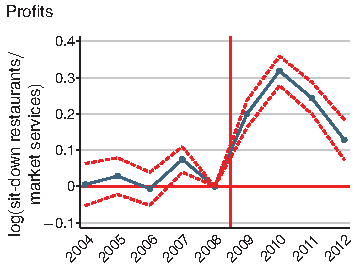
\includegraphics[width=15cm]{Figure1.pdf}
  \caption{关于对数利润的事件研究系数$\{\beta_s\}$}
\end{figure}

\begin{figure}[htbp!]
  \centering
  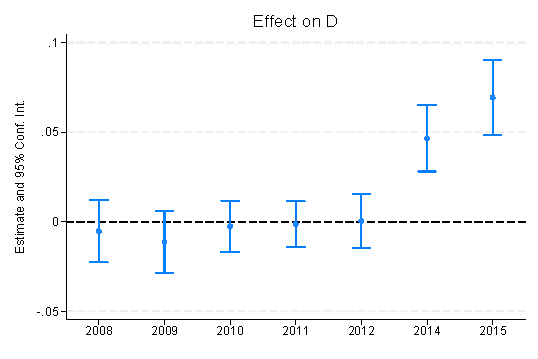
\includegraphics[width=15cm]{Figure2.pdf}
  \caption{敏感性分析}
\end{figure}

\newpage

\nocite{Andrews2023inference}
\nocite{benzarti2019really}
\nocite{callaway2021difference}
\nocite{goodman2021difference}
\nocite{rambachan2023more}
\nocite{roth2022pretest}
\nocite{roth2023s}
\nocite{sun2021estimating}
\nocite{Zhang2023}
\printbibliography[heading=bibintoc, title=\ebibname]

\end{document} 